\documentclass[11pt, oneside]{article} 
\usepackage{geometry}
\geometry{letterpaper} 
\usepackage{graphicx}
	
\usepackage{amssymb}
\usepackage{amsmath}
\usepackage{parskip}
\usepackage{color}
\usepackage{hyperref}

\graphicspath{{/Users/telliott/Github/calculus_book/png/}}
% \begin{center} 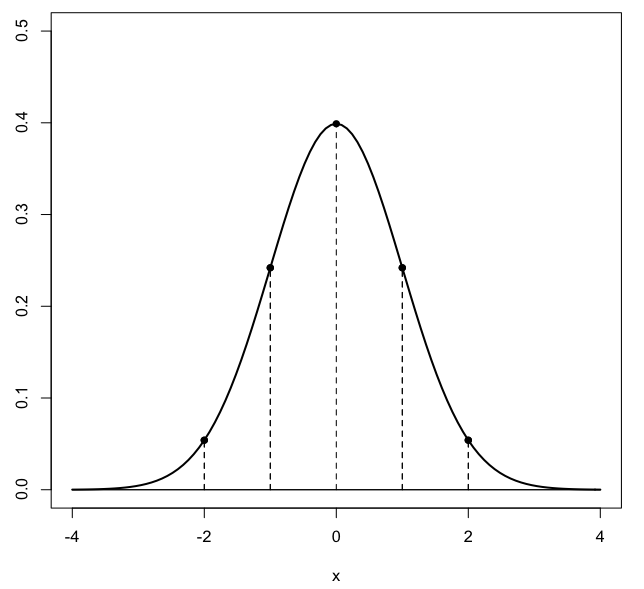
\includegraphics [scale=0.4] {gauss3.png} \end{center}

\title{Introduction}
\date{}

\begin{document}
\maketitle
\Large

\label{sec:Value_of_pi}

\section*{Archimedes and $\pi$}
Since Archimedes is a strong presence in this book, we will discuss his method for approximating the value of $\pi$, the ratio of the circumference of a circle to its diameter.  The commonly cited result is 

\begin{quote}The ratio of the circumference of any circle to its diameter is less than 3 1/7 but greater than 3 10/71.\end{quote}

In decimal that is $3.140845.. < \pi < 3.1428571$.

However, to some extent this misses the main idea, that Archimedes described an iterative procedure which can be used to calculate the value of $\pi$ \emph{to any desired accuracy}.

Although the idea is beautiful, his argument is somewhat unwieldy in detail, so instead we will use modern trigonometry to achieve the same result more economically.  

For a discussion of Archimedes actual method (based on a translation by Heath), see this web page

\url{https://itech.fgcu.edu/faculty/clindsey/mhf4404/archimedes/archimedes.html}

and I have worked out the same proof in detail in this \hyperref[sec:Archimedes_and_pi]{\textbf{chapter}}.

In addition, we will connect the trigonometry to easy formulas for the perimeter and area of inscribed and circumscribed polygons.  The first part is in this chapter, and the second part has been split out into another \hyperref[sec:Gregory]{\textbf{chapter}}, which is in the Addendum.

If this material is too esoteric, it can be skipped without loss of continuity in the rest of the book.

I should also point out that although we don't follow Archimedes exactly, a key element which he relies upon is the proof that, for an angle bisector in a right triangle, the adjacent sides are in the same proportion as the two segments formed where the bisector meets the other side.

\begin{center} 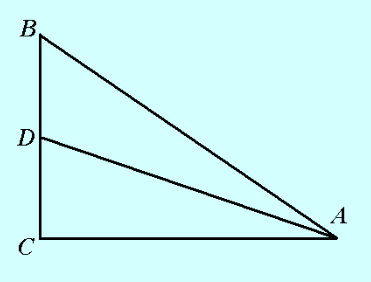
\includegraphics [scale=0.4] {angle_bisector.png} \end{center}
Here:  
\[ \frac{AB}{AC} = \frac{BD}{DC}  \]
We showed a proof of this earlier (\hyperref[sec:angle_bisector]{\textbf{here}}).

\subsection*{the method}

We will approximate the value of $\pi$ by squeezing it between the perimeter of an inscribed polygon, which is less than the circumference of the circle, and the perimeter of a circumscribed polygon, which is greater than the circumference of the circle.  
\begin{center} 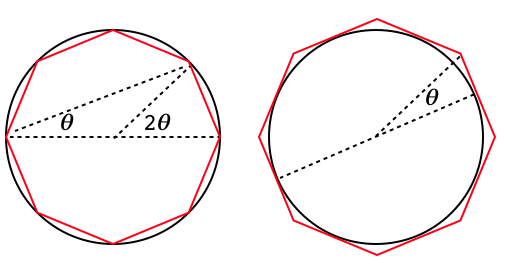
\includegraphics [scale=0.5] {pi.png} \end{center}

We use a circle of \emph{diameter} equal to $1$ (rather than the radius, which is more usual).  The circumference of the circle is then equal to $\pi$, the value which gets squeezed between the two perimeters.

The figure shows a sketch of the polygons when $n=8$.  We will be increasing the number of sides by a factor of $2$ at each step, so these are really $2^n$-gons with $n=3$ here.

\subsection*{Finding perimeters in terms of angle $\theta$}
For the left panel, we have $8$ sides, so the central angle (marked $2\theta$) is equal to
\[  \frac{2 \pi}{8} = \frac{\pi}{4} = 45^\circ \]
and $\theta$ is one-half that.  

\begin{center} 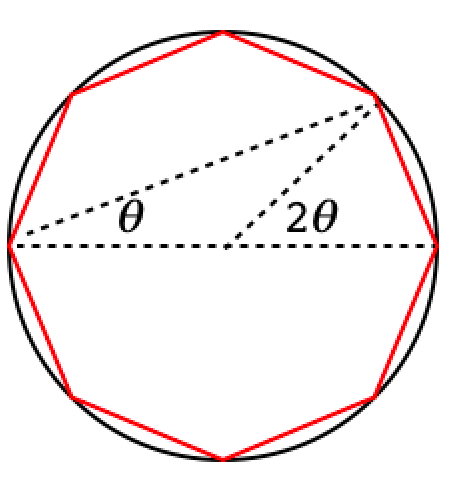
\includegraphics [scale=0.3] {piL.png} \end{center}
By a standard theorem (from Thales), the triangle above containing angle $\theta$, with the diameter as one side, and two other vertices also on the circle, is a right triangle.  The inscribed n-gon side of length $S$ (shown in red) is equal to $\sin \theta$, since the hypotenuse of the triangle is the diameter of the circle, which is equal to $1$.  

The total perimeter is $8 \cdot S$.

[Alternatively, use half the angle at the center of the circle (i.e. $\theta$).  Then half the length of the red line $S/2$, divided by the radius ($r = 1/2$) gives $S = \sin \theta$, the same result.]

For the right panel, we have the same circle (now showing the outside polygon, circumscribing the circle), it is just rotated slightly..  One dashed line extends a bit further to the vertex of the n-gon outside.  The angle marked $\theta$ is one-half the angle we marked as $2 \theta$ previously since now the diameter comes down to the middle of the side.

We compute the whole length of the side $T$ as follows.  The half-side is $T/2$ and the hypotenuse of the triangle is one-half the unit diameter, which is $1/2$, so $T = \tan \theta$.  The total perimeter is $8 \cdot T$.

\begin{center} 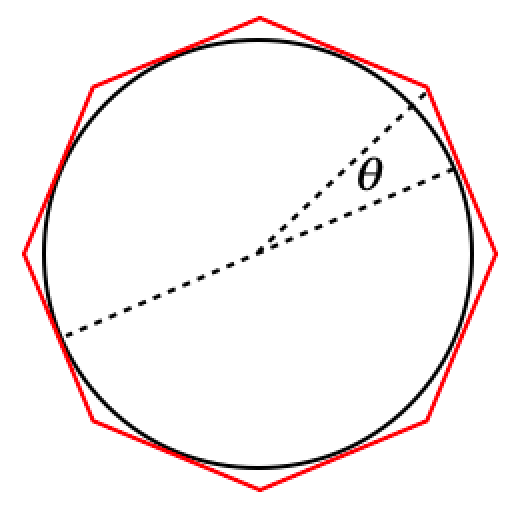
\includegraphics [scale=0.3] {piR.png} \end{center}
All of this gives us two simple equations for the two perimeters.  At each stage there are $2^n$ sides, the length of each short side $S$ on the inside equals $\sin \theta$ and the length of each short side on the outside $T$ is equal to $\tan \theta$, where $\theta = 2 \pi/2^n$.

The total length of the inside perimeter is $nS = n \sin \theta$ and that of the outside is $nT = n \tan \theta$.  When we go from $\theta$ to $\theta/2$ and $n$ to $2n$, we must compute the new values $S'$ and $T'$ from $S$ and $T$ using the half-angle formulas, and then also multiply by 2 to take account of the change from $n$ to $2n$ for the total circumference.

\subsection*{The base case}
If we go back to the square ($n=2, 2^n = 4$), then the angle $\theta$ is $\pi/4$.

The tangent is $T = \tan \pi/4 = 1$ and the sine is $S = \sin \pi/4 = 1/\sqrt{2}$.  

Our formulas say that on the inside, the perimeter is $4S = 4/\sqrt{2} = 2 \sqrt{2}$ and on the outside, the perimeter is $4T = 4$.  

From simple geometry, we can calculate that the circumscribing square has a side length which is twice the radius of the circle, that is, $1$ for our  circle with unit diameter, so its perimeter is $4$, which checks.

Similarly, an inscribed square can be decomposed into four isosceles right triangles with sides of length $1/2$ and hypotenuse $1/\sqrt{2}$, so the total perimeter is $4/\sqrt{2}$, which also checks.

Now, what we are going to do is to increase $n$ in steps of 1, that increases $2^n$ by a factor of $2^1 = 2$ each time.  Doubling $n$ halves the angle.  So all we need is a way to compute trigonometric functions of $\theta/2$, knowing the values for $\theta$, so we can calculate what happens to the perimeter.  We already know how to do that.

\subsection*{Half angle formulas}

We have derived these elsewhere.  Refer to this \hyperref[sec:double_half_angles]{\textbf{chapter}}.

The unprimed values refer to angle $\theta$, while the primed ones have angle $\theta/2$.

\[ C' = \sqrt{\frac{1}{2} (1 + C)}  \]
This can be rearranged (e.g.) to give $2[C']^2 = 1 + C$, which we'll use in a second.

\[ S' = \frac{S}{2 C'} \]

\[ T' = \frac{S'}{C'} = \frac{S}{2 [C']^2} \]
\[  = \frac{S}{1 + C} \]

So, given $S, C$ and $T$, first calculate $C'$ and $T'$ and then $S'$.  To get the perimeters, remember that factor of two from doubling $n$, the number of sides.

\subsection*{another approach}

This web page originally got me started with this derivation

\url{http://personal.bgsu.edu/~carother/pi/Pi3d.html}

(Unfortunately, the link is dead now, probably because the University took Dr. Carother's pages down when he died, idiots).  It has been preserved by the wayback machine:

\url{https://web.archive.org/web/20171024182015/http://personal.bgsu.edu/~carother/pi/Pi3d.html}

On that page, there was given an arguably simpler pair of formulas listed, namely, for an inside perimeter $p$ and an outside perimeter $P$
\[ P' = \frac{2pP}{p + P} \]
\[ p' = \sqrt{pP'} \]

The first equation can be rearranged to give
\[ \frac{1}{P'} = \frac{1}{2} \ [ \frac{1}{P} + \frac{1}{p} \ ] \]
which is the definition of the harmonic mean of $p$ and $P$, while the second equation is the geometric mean.

Since in our derivation $p$ and $P$ are the same multiple of $S$ and $T$, it seems like the same relationships should hold for the sine and tangent, but we must remember the extra factor of $2$.

From the half-angle formulas, we said that
\[ T'  = \frac{S}{1 + C} \]
Multiply top and bottom on the right by $T$:
\[ T' = \frac{ST}{T + S} \]

Recall that $S$ is the same as $p$, within a factor of $n$, and that $T$ is the same as $P$, within the same factor.
\[ p = nS \]
\[ P = nT \]
while 
\[ P' = 2nT' \]

Going back to 
\[ T' = \frac{ST}{T + S} \]
\[ 2nT' = \frac{2 \cdot nS \cdot nT}{nT + nS} \]
\[ P' = \frac{2pP}{p + P} \]

This is what was given.

For the second one
\[ S' = \frac{S}{2 C'} \]
\[ = \frac{S}{2} \ \frac{T'}{S'} \]
Then
\[ 4[S']^2 = S \cdot 2T' \]
\[ [2nS']^2 = nS \cdot 2nT' \]
Changing  variables, $p' = 2nS'$
\[ [p']^2 = pP' \]

Finally
\[ p' = \sqrt{pP'} \]
which matches what was given.

\subsection*{Calculation}

Let's run a simulation to see what kind of numbers we get.  Start with the square ($n=2$, $2^n = 4$)
Previously we found that $S=1/\sqrt{2}$ and $T=1$ so
\[ p = 2^n S = \frac{4}{\sqrt{2}} = 2.8284 \]
\[ P = 2^n T = 4 \]
Let's try a script to calculate this to larger $n$.

\url{https://gist.github.com/telliott99/19f521c807210171a4847b319104b3df}

\begin{verbatim}        
Output:

> python pi.py
 2 2.8284271247  4.0000000000
 3 3.0614674589  3.3137084990
 4 3.1214451523  3.1825978781
 5 3.1365484905  3.1517249074
 6 3.1403311570  3.1441183852
 7 3.1412772509  3.1422236299
 8 3.1415138011  3.1417503692
 9 3.1415729404  3.1416320807
10 3.1415877253  3.1416025103
11 3.1415914215  3.1415951177
12 3.1415923456  3.1415932696
13 3.1415925766  3.1415928076
14 3.1415926343  3.1415926921
15 3.1415926488  3.1415926632
16 3.1415926524  3.1415926560
17 3.1415926533  3.1415926542
18 3.1415926535  3.1415926537
19 3.1415926536  3.1415926536
> 
\end{verbatim}

That looks pretty good to me, although it's a bit slow to converge.

This is really quite amazing.  Archimedes has not only calculated $\pi$ to 3 significant figures.  More important, he has provided us with an iterative procedure that can be used to calculate the value to \emph{any precision we desire}.  As an engineer, Archimedes knew that $3.1416$ is precise enough, so he stopped.

After all, no one wants to be William Shanks, or one of these guys:

%\url{https://en.wikipedia.org/wiki/Chronology_of_computation_of_π}

Quote:

\begin{quote}[He] calculated pi to [n] digits, but \emph{not all were correct.}\end{quote}

There is an additional \hyperref[sec:Gregory]{\textbf{chapter}} which substantially extends the above discussion, showing a geometric derivation of the basic relationships and developing new formulas involving the areas as well as the perimeters of the sectors of inscribed and circumscribed polygons.

\subsection*{area}
I became aware later that there is yet another way to apply the method, and that is to calculate the \emph{areas} of inscribed and circumscribed polygons.  We'll go through this briefly.

For this approach we use a unit circle (radius $1$) rather than a diameter of $1$, as we did above.  As before, we define $\theta$ to be the central angle of the half-sector (i.e. $\theta = 2\pi/2n$).
\begin{center} 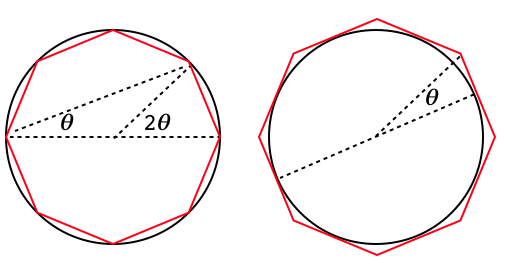
\includegraphics [scale=0.5] {pi.png} \end{center}
Rather than draw an entirely new figure, just imagine in the left panel that we draw the angle bisector of angle $2 \theta$.  The area of each new triangle is then $\sin \theta \cos \theta / 2$ and the total area of the inner polygon is
\[ a = n \sin \theta \cos \theta = n SC \]
in the notation we adopted previously in this chapter.  And, as before, to progress to $a'$ we have a factor of $2$ as well as the new values $S'$ and $C'$:
\[ a' = 2n S'C' \]

For the circumscribed or outer polygon, we just have what we had before, that the side length of the triangle in the right panel is $\tan \theta$ so the total area is
\[ A = nT \]

Bring in the half-angle formulas as follows:
\[ a' = 2n S'C' = 2n \cdot \frac{S}{2C'} \cdot C' = nS \]
That is slick, but we need an expression for $nS$:
\[ aA = nSC \cdot n \frac{S}{C} = [nS]^2 \]
\[ aA = [a']^2 \]
\[ a' = \sqrt{aA} \]

This is like, and yet subtly different than what we had when calculating the perimeter.

Since
\[ A = nT \]
and
\[ A' = 2nT' \]
\[ = 2n \frac{ST}{S + T} = 2 \frac{nS \cdot nT}{nS + nT} \]
\[ A' = 2 \frac{a'A}{a' + A} \]
Compare
\[ a' = \sqrt{aA}  \ \ \ \ \  A' = 2 \frac{a'A}{a' + A} \]
\[ p' = \sqrt{pP'}  \ \ \ \ \   P' = 2 \frac{pP}{p + P} \]

However, it turns out that when you take account of the differing size of the circle for perimeter and area methods, and thus the initial values of $p,P,a$ and $A$, the different order of operations results in precisely the same calculation.

\end{document}